% easychair.tex,v 3.5 2017/03/15

\documentclass{easychair}
%\documentclass[EPiC]{easychair}
%\documentclass[EPiCempty]{easychair}
%\documentclass[debug]{easychair}
%\documentclass[verbose]{easychair}
%\documentclass[notimes]{easychair}
%\documentclass[withtimes]{easychair}
%\documentclass[a4paper]{easychair}
%\documentclass[letterpaper]{easychair}

\usepackage{doc}

% use this if you have a long article and want to create an index
% \usepackage{makeidx}
\usepackage{hyperref}% http://ctan.org/pkg/hyperref
\hypersetup{%
  colorlinks = true,
  linkcolor  = black
}
% In order to save space or manage large tables or figures in a
% landcape-like text, you can use the rotating and pdflscape
% packages. Uncomment the desired from the below.
%
% \usepackage{rotating}
% \usepackage{pdflscape}
\usepackage{textcomp}
% Some of our commands for this guide.
%
\newcommand{\easychair}{\textsf{easychair}}
\newcommand{\miktex}{MiK{\TeX}}
\newcommand{\texniccenter}{{\TeX}nicCenter}
\newcommand{\makefile}{\texttt{Makefile}}
\newcommand{\latexeditor}{LEd}

%\makeindex

%% Front Matter
%%
% Regular title as in the article class.
%
\title{Extending domain name monitoring. 
Identifying potential malicious domains using hash signatures of DOM elements
}

% Authors are joined by \and. Their affiliations are given by \inst, which indexes
% into the list defined using \institute
%
\author{
Andrea Bernardini\inst{1}
}

% Institutes for affiliations are also joined by \and,
\institute{
  Fondazione Ugo Bordoni, Rome, Italy\\
  \email{abernardini@fub.it}
}

%  \authorrunning{} has to be set for the shorter version of the authors' names;
% otherwise a warning will be rendered in the running heads. When processed by
% EasyChair, this command is mandatory: a document without \authorrunning
% will be rejected by EasyChair

\authorrunning{}

% \titlerunning{} has to be set to either the main title or its shorter
% version for the running heads. When processed by
% EasyChair, this command is mandatory: a document without \titlerunning
% will be rejected by EasyChair
\titlerunning{}

\begin{document}

\maketitle

\begin{abstract}
  The usage of disposable domains for malicious activities is an increasing trend and a fertile ground for fraudsters actions from phishing to fake goods selling. Those domains are registered daily, go online within a few hours and last for a very short time. Due to the existence of automated developing tools for content creation and efficient site management, a single monicker entity may be in charge of large networks of thousands of domains. Such a grade of automation requires the usage of easy transmutable websites templates and repetitive code snippets. In order to deploy a more resilient anti-fraudster strategy, we present a framework which combines web pages scraping procedures, simhash fingerprint based near duplicate document detection and agglomerative clustering. 
The objective is twofold: firstly to identify common and repetitive structural patterns in potential illicit websites; secondly to monitor new emerging technical trends in short period time frames. The framework has been tested on a corpus of newly registered .com domains for a period of three weeks. The results consistently confirm the existence of recurring technical schemes. We showed that, by using document fingerprinting, it considerably increases the overall comprehension of strategies used in complex suspicious domains networks and it may be of support for a new concept of domain protection.

\end{abstract}

% The table of contents below is added for your convenience. Please do not use
% the table of contents if you are preparing your paper for publication in the
% EPiC Series or Kalpa Publications series

\setcounter{tocdepth}{2}
{\small
\tableofcontents}

%\section{To mention}
%
%Processing in EasyChair - number of pages.
%
%Examples of how EasyChair processes papers. Caveats (replacement of EC
%class, errors).

%------------------------------------------------------------------------------
\section{Context}
\label{sect:Context}

Thousands of domains are registered and dropped every day across all top-level domains. The second quarter of 2017 closed with approximately 332 million of registration and it is an increasing number quarter by quarter~\cite{dnib}. The registered domains are completely new or could be expired/deleted recently. Malicious entities use to register domains daily for creating complex networks with the objective of generating spam, promoting and selling fake goods or induce users in phishing~\cite{Cova:2008:NFP:1496702.1496706}~\cite{europol}. 
Often a single entity (person or organization) is in charge of a complex network of interconnected domains, hosted in various countries. The life cycle of such domains may range from few days to years depending on the responsiveness of potential victims, of the targeted brands and controlling authorities.  It may occur that those domains are finally inserted in a DNS Blacklists~\cite{opendns}, be mentioned in sites contrasting scam and phishing~\cite{phishtank} or be removed by search engine indexing system. The loss of a domain due DNS block or removal by search engine has negligible effects. A new domain can be quickly registered, and a new site can be deployed. Indeed, all the procedures for managing contents can be executed by toolkits~\cite{blackhat} able to clone templates and randomize contents producing web pages similar or identical. Recent studies~\cite{Carpineto:2017:LDM:3106426.3106441}~\cite{Wadleigh:2015:EML:2736277.2741658} focus on asserting the trustworthiness of websites by the analysis of search engine results on the base of a range of features extracted from pages and integrated eventually with external resources as domain registration data and other metrics.
In this work, we focus on the detection of potential illicit websites by identification of anomalous density of structural similarities on newly registered websites. The usage of management toolkits and templates leave often traces and technical marks. Based on this observation we tackle the problem of identification of potentially malicious sites to a well-known research topic as the nearly duplicate document detection applied to web pages document structure. 
\\
The rest of the paper is structured as follows:

\begin{enumerate}
\setcounter{enumi}{1}
\item
Introduction reviews the related works and summarize some main concepts;

\item
Proposed approach describes the proposed framework and its three main components;

\item
Experimental setup describes the settings and the data corpus;

\item
Results and observations

\item
Conclusions 

\end{enumerate}




%------------------------------------------------------------------------------
\section{Introduction}
\label{sect:Introduction}

Duplicated and mirrored web pages are seen in plenty in the World Wide Web, and they have been object of studies for as long as the web exists as its overlap with many topics as plagiarism detection, spam detection and even crawlers optimization. The field of near-duplicate document (NDD) detection focuses on the individuation of almost identical documents which differ in small portions. In the context of web pages the differences could be in the text, in the images, as well as in the structure. More in detail a web page may be decomposed in different layers of features: semantic, structural, and visual. 
\begin{itemize}
  \item The semantic layer of a page is the information and the topics it expresses;
  \item The structural layer of a page is the underlying skeleton of a page;
  \item The visual layer of a page represents the visual information conveyed by the page.
\end{itemize}


In general, all the approaches of NDD vary on the strategy for the document features selection, for the compression of the features in a signature, for the comparison the documents with a similarity measures and for the corpus under consideration. The growing size of datasets and the high-dimensional space of documents leaded to the necessity of investigating dimensionally reduction techniques. Broder~\cite{Broder:1997:SCW:283554.283370} introduced the algorithm MinHash and a technique called ‘shingling’ used for the estimation of document resemblance based on the overlapping of a subset of adjacent words sequences (called shingles). The MinHash is the first of a more general framework of algorithms, the Locality Sensitive Hashing~\cite{lsh} devised for solving near duplicate and similarity problems for web pages and images~\cite{Indyk:1998:ANN:276698.276876}~\cite{7840807}. Broder studies have been reviewed to investigate the evolution of individual pages and subsequently related clusters of near-duplicates pages. It emerged that two documents that are near-duplicates of one another are very likely to still be near-duplicates after months ~\cite{Fetterly:2003:ECN:951953.952397}. MinHash was at first applied to a set of 30 million web pages, but the dimension of dataset kept growing, so optimization techniques were investigated. 
Charikar~\cite{Charikar:2002:SET:509907.509965} proposed a fingerprinting techniques on documents for mapping high dimensional vectors to small-sized fingerprints. The process is organized in two steps. Firstly, for each document it is calculated a representative hash and then near duplicates are detected by identifying documents that have similar hashes. Manku~\cite{Manku:2007:DNW:1242572.1242592} demonstrated the goodness of Charikar\textquotesingle s  technique and proposed an algorithm for identification of fingerprints which differ from a chosen one for a maximum of k positions. Other studies focused on the performance respect to the overall complexity of the analysis ~\cite{key:article}. Narayana proposed an approach working on keyword extraction and the correlation between two documents it is given if the similarity score is greater than a threshold ~\cite{Narayana:2010:FTE:1947599.1947616}. Other mixed approaches have been proposed.~\cite{kumar2013near} proposed a mixed approach of keywords extraction and fingerprinting. Most of those studies concentrate on a vector based on semantic features, the text contained in the page. All other page components as the HTML markup tags are substituted by whitespaces. In the study~\cite{7785739} the structural similarity of documents based on the Tree Edit Distance between Document object model (DOM)~\cite{w3c} trees is investigated. Recent studies explore the combination of LSH techniques with clustering process~\cite{koga2007fast} to reduce computational costs working on only semantic layer or a mixed semantic and structural layer, which joins content and other data as title, description, keywords, and tags~\cite{7840807}




\section{Proposed approach}
\label{sect:Proposed approach}

In our proposed approach we focus on the analysis of structural layer features of web pages, extracting from an HTML page the corresponding DOM tree and transforming it in a stripped version, containing only HTML tags, by the removal of all textual contents. 
The sequence of tags is then converted, using the simhash algorithm, in hashed fingerprints. Due to the properties of simhash algorithm similar documents have similar fingerprints so it is possible to group fingerprints in hash buckets and then store them in hash tables. 
The similarity is calculated by using the Hamming~\cite{6772729} distance since we converted the document features space to a hash f-bit space. Subsequently, we randomly select from each bucket candidates for nearly duplicate selection, and we construct, by the resulting aggregations, clusters of similar documents. The system architecture is composed of three main components as described in fig.~\ref{fig:1} .

\begin{figure}[ht]
  \begin{centering}
  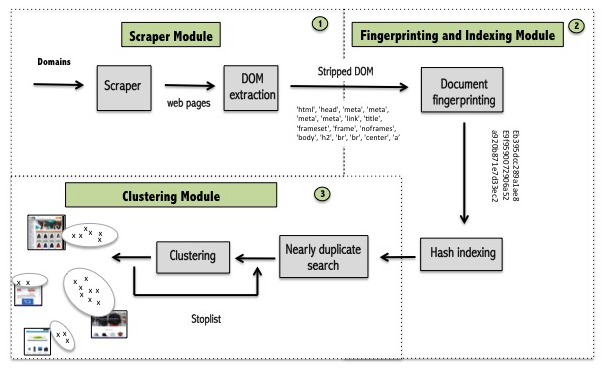
\includegraphics[width=0.5\textwidth]{1.png}
  \caption{System Architecture}
  \label{fig:1}
  \end{centering}
\end{figure}

\subsection{Scraper module}
\label{sect:Scraper module}

The scraper module is in charge of the preprocessing activity consisting in the page selection, crawling and parsing. The scraper module makes usage of various scraping tools as cURL~\cite{curl}, a library as Beautiful Soup~\cite{bs4} and a headless browser as Selenium~\cite{selenium} to access web pages. The selection consists of accessing the daily newly registered domains lists and choosing the domains containing terms belonging to the bag of word in the url. Crawling consist of establish communication with the correspondent domain through the HTTP protocol and, in case of reachability, digest (download) the domain homepage. Web pages are based on an underlying object structure, namely, the DOM. The DOM is a cross-platform and language-independent application programming interface that treats an HTML, XHTML, or XML document as a tree structure (fig.~\ref{fig:DOM Tree} ) where each node is an object representing a part of the document. The DOM defines the logical structure of documents and the way a document is accessed and manipulated.

\begin{figure}[ht]
  \begin{centering}
  
\includegraphics[width=0.5\textwidth]{2.png}
  \caption{DOM Tree}
  \label{fig:DOM Tree}
  \end{centering}
\end{figure}

Stripping procedure is a transformation which manipulates the crawled document, removes contents and terms not of interest to obtain a linear stripped DOM tree. Consequently, all pages contents, all the tag attributes are ignored.  as for example in 
\\\textit{[‘html', 'head', 'meta', 'meta', 'meta', 'meta', 'link', 'title', 'frameset', 'frame', 'noframes', 'body', 'h2', 'br', 'br', 'center', 'a',..]}

%------------------------------------------------------------------------------
\subsection{Fingerprinting and Indexing module}
\label{sect:Fingerprinting and Indexing module}

A fingerprinting hashing algorithm is a transformation that maps an arbitrarily large data item (in this paper, we refer as items to web pages) to a much shorter bit string that is likely to identify the original data. More formally, let’s introduce H as a family of hashing functions h mapping an input x to a compact code y as y = h(x).

In our case we opted for a family H of transformations, the locality sensitive hashing which let the generated fingerprints to maintain an internal similarity even in case of an item small change. It means that a similar set of item in the domain of these functions have a higher probability of colliding in the range space than dissimilar ones. More formally an LSH~\cite{lsh} family F is defined for a metric space M=(M,d), and an approximation factor c \begin{math} > \end{math} 1. This family of function F is a family of functions h: M -\begin{math} > \end{math} S which map elements from the metric space to a bucket s ϵ S . The LSH family satisfies the following conditions for any two points p, q ϵ M , using a function h ϵ F which is chosen uniformly at random:

  \begin{itemize}
  \item if d(p,q) ≤ R then h(p) = h(q) (i.e. p and q collide)  with probability at least P1
  \item if d(p,q) \begin{math} \geq \end{math} cR , then h(p)=h(q) with probability at most P2
  \end{itemize}

    
A family of function is of interest when P1 \begin{math} > \end{math} P2 . Such a family F is called (R, cR, P1, P2 ) -sensitive. For the objectives of this research, we identified Charickar\textquotesingle s simhash algorithm~\cite{Charikar:2002:SET:509907.509965}
 as an appropriate algorithm for fingerprint generation. The advantage of this algorithm is the compression of high dimensional documents to small sized fingerprints of a chosen size, traditionally 64 bits. So a standard web pages of hundreds of KB size is firstly linearized to a stripped DOM version and then the correspondent fingerprint is generated with the simhash algorithm (Table~\ref{tab:table1}). 



\begin{table}[htp]
  \begin{centering}
    \begin{tabular}{lrrrrrrrr}
    \hline
    Domain            & Fingerprint  \\
                          
    \hline
    Domain 1 &  eb395dcc289a1ae8   \\
    \hline
    Domain 2      &  e9f9590072906a52   \\
	
    \hline
    Domain 3      &  a920b871e7d33ec2   \\
    
    \hline
    \end{tabular}
    \caption{Registering time frame for a multi-term cluster of domains }
    \label{tab:table1}
  \end{centering}
\end{table}

Lastly the fingerprints are indexed using hash tables, formed by storing the items with similar codes in hash buckets.


%------------------------------------------------------------------------------
\subsection{Clustering module}
\label{sect:Clustering module}

After creating a compact signature for documents and hashing them in hash tables, a way to efficiently compute a similarity measure for constructing clusters of homogeneous documents, has now to be found. 
More formally, given a set of hash items X = { $x_1$  .. $x_n$} and given a query item q in {$q_1$ .. $q_m$ } the goal is to find the closest points to q in X  as candidates for building up clusters. As similarity measure between hash items, we use the Hamming distance. Given a set of items hash X, we define the Hamming distance between two items $x_1$, $x_2$ to be the number of components in which they differ. As an example in a cluster C containing ($x_1$ = 00011001, $x_2$ = 00010011), the Hamming distance H($x_1$,$x_2$) = 2 because the bit-hash differs in the 5th and 7th positions. 
While fingerprinting allows to computer quickly and efficiently the resemblance of two documents, it does not solve the computational issue of considering all possible pairs. However, the locality sensitive property of LSH implies that similar items have a larger probability to be mapped to the same bucket than dissimilar items, so for a query instance x, it can be used for a first approximation the instances stored in buckets containing x. From each of the hash buckets we randomly choose an item as query item qi for a similarity search. 
This search can be executed efficiently as search of all fingerprints that differ from a given fingerprint in at most k bit positions, where k is a small integer (Manku, 2007). The results are then aggregated using an agglomerative clustering technique where elements are merged into the cluster until the similarity condition is respected.

%------------------------------------------------------------------------------
\section{Experimental setups}
\label{sect:Experimental setups}

The computer used for the experiments is an IMac, with 3.4 GHz intel Core I7 with 16 GB of ram. The Data Corpus has been generated from the daily list of registered .com domains in the month of September 2017. The daily list contains an average of 100K domains a day with peaks during the working days and cusps during weekend. 
For the purposes of this research, we oriented on potential counterfeiting domains by using a bag of words of interest containing both fashion brands and transactional terms as it follows:\\

{\textit{Bag of words =  {louboutin, iceberg, armani, gucci, hogan, iceberg, vuitton, prada, tods, moncler, nike, adidas, sales, outlet, ferragamo}.}}
\\

Then the newly registered domains were filtered on the base of the bag of words and a daily monitoring of resulting domains were executed for a period of three weeks. Globally 4000 domains have been monitored. 

\section{Results and observations}
\label{sect:Results and observations}

A simhash fingerprints dimension of 64 bits was used for the experiment. For the corresponding value of k, the tolerated bit positions range between similar fingerprint, we evaluated a range from 1 to 5. It is clear that boosting the value of k implies an increasing tolerance of differences between fingerprints and the gathering of items structurally more different. The value of k is directly proportional to the number of multi-item clusters (2 or more items) and inversely proportional to the number of clusters containing one unique item (fig.~\ref{fig:3}). Subsequently a reduced number of clusters are generated and it is altered the distribution of items within a cluster.

\begin{figure}[ht]
  \begin{centering}
  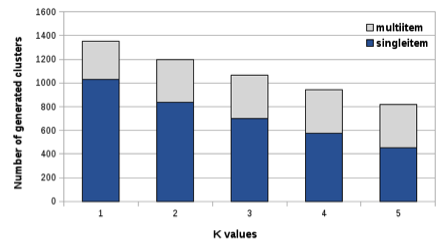
\includegraphics[width=0.5\textwidth]{3.png}
  \caption{Value of k  and cluster single-item, multi-item distribution}
  \label{fig:3}
  \end{centering}
\end{figure}

For choosing the correct value of k, we computed two internal measures: cohesion (how closely related are the items in a cluster) and separation (the distinctiveness of a cluster from the others) using the fingerprint with a higher similarity with all the other fingerprints within the cluster, as the centroid of a cluster. Results indicate a reasonable value of k=3 as already evidenced in other studies~\cite{Manku:2007:DNW:1242572.1242592}.

To compute the appropriateness of data partitions we manually inspected the clusters by visual analysis and source code inspection.
Two experts labeled the true positives(tp),the decision assigns two similar documents to the same cluster, and false positives(fp), the decision to assigns two dissimilar documents to the same cluster.
Two misleading results were noticed. Firstly, some javascript injected pages were not processed correctly, as in the case of specific web pages building platforms as vix.com or leadpages.net, and it led to the creation of few high-density clusters. For maintaining a reasonable computational time we did not further investigate domains sharing those fingerprints as it would require a much higher scraping time. We either noticed that in case of sites not yet published, due the freshness of newly registered domains, the framework analyzed and clustered the corresponding parking pages (the placeholder for a newly registered domain before a website is ready for launching) for services as \textit{godaddy.com}, \textit{a2hosting}  and so on. 

We then calculated the measure of precision, the percent of positive predictions, as it follows:

\[
    Precision = \frac{tp}{tp + fp}
\]

From this measure(Table~\ref{tab:table5}), it  appears that, the proposed framework performs well, in the case of traditional web pages, creating homogeneous clusters.

\begin{table}[htp]
  \begin{centering}
    \begin{tabular}{lrrrrrrrr}
    \hline
    Typology           & Precision \\
    
    \hline
    Parking pages      &  0,940066593	   \\
       
    Javascript injected pages      &  0,916666667	   \\
    
   
    Traditional web pages      &  0,847250509   \\

    \hline
    \end{tabular}
    \caption{Cluster precision by page typology }
    \label{tab:table5}
  \end{centering}
\end{table}


The fingerprints of parking pages and javascript injected pages, corresponding to nearly the 55\% of the total clusters, were inserted in a stoplist and removed at the successive clustering phase. In fig.~\ref{fig:4} the clusters occurrence by cluster size.

\begin{figure}[ht]
  \begin{centering}
  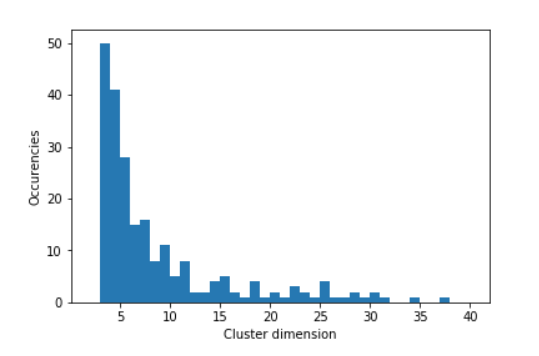
\includegraphics[width=0.5\textwidth]{4.png}
  \caption{Cluster size and occurrence}
  \label{fig:4}
  \end{centering}
\end{figure}

We then switched to corresponding domains url to investigate the distribution of terms within the clusters. By the comparison of terms from our bag of words and the domains urls, we then proceeded to separate clusters related to one term i.e. “single-term cluster” from clusters related to more than one term i.e. “multi-term clusters”. A single-term cluster contains fingerprints of domains related to only one term of the bag of words as \textit{loveinnike.com}, \textit{hotnike.com}, \textit{uknike.com}  with \textit{nike} as term. A multi-term cluster contain fingerprints of domains related to two or more term from the bag of words as \textit{pradashoes.com}, \textit{nikempire.com}, \textit{moncletcoat2019.com} with \textit{nike, prada, moncler} as terms. It results, with such segmentation, a partition of 109 multi-item single-term clusters and 73 multi-item multi-term clusters. 

The results of single-term cluster analysis reinforce the traditional brand domain monitoring analysis, which works mainly on lexical similarity, offering both a measure of a lexical and structural similarity (fig.~\ref{fig:5}).

\begin{figure}[ht]
  \begin{centering}
  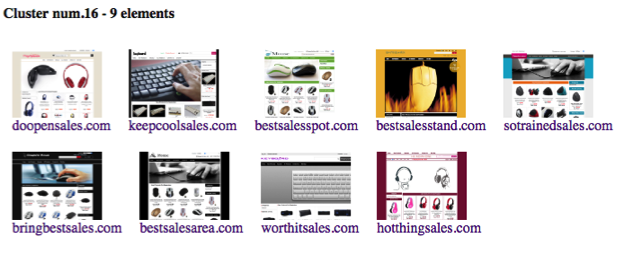
\includegraphics[width=0.5\textwidth]{5.png}
  \caption{Items from single-term cluster sales}
  \label{fig:5}
  \end{centering}
\end{figure}

	The results of multi-terms cluster analysis leads to the discovery of not obvious connections between domains based on the usage of similar structured templates. In fig.~\ref{fig:6} an example of two domains registered on the same day without any lexical url similarity, promoting different products using different keywords, were clustered together due the usage of a nearly similar structural layer. 
\begin{figure}[ht]
  \begin{centering}
  
\includegraphics[width=0.5\textwidth]{6.png}
  \caption{Items from a multi-terms cluster}
  \label{fig:6}
  \end{centering}
\end{figure}


\begin{table}[htp]
  \begin{centering}
    \begin{tabular}{lrrrrrrrr}
    \hline
    Domain name           & Created on & Updated on \\
                          
    \hline
    hotthingsales.com       &  2017-09-18T06:42:58Z & 2017-09-18T07:11:46Z  \\
   
    worthitsales.com      &  2017-09-18T06:43:02Z & 2017-09-18T07:11:51Z  \\
    

       bringbestsales.com   & 2017-09-18T06:43:03Z  &  2017-09-18T07:11:45Z \\
    
      doopensales.com    & 2017-09-18T06:43:04Z  &  2017-09-18T07:11:38Z \\
   
      keepcoolsales.com    & 2017-09-18T06:43:15Z  &  2017-09-18T07:11:45Z  \\
    
       sotrainedsales.com    &  2017-08-29T09:14:12Z & 2017-08-30T00:57:47Z   \\
  
        bestsalesspot.com  & 2017-08-29T09:14:21Z  & 2017-08-30T00:57:42Z  \\
  
    
    
        bestsalesstand.com  &  2017-08-29T09:14:43Z & 2017-08-30T00:57:42Z   \\
    \hline  
    
    \end{tabular}
    \caption{Registering time frame for a single-term cluster of domains }
    \label{tab:table2}
  \end{centering}
\end{table}


We then reassessed clusters results taking in account the time variable. For each domain the time of registration and update was extracted using a whois service. A correlation both on structural similarities and domain registration timing could be a direct indication of the usage of automated bulk publishing tools and an indirect confirmation of the affiliation to a moniker domains network. Preliminary results confirm this correlation and indicate the usage of bulk registering tools. Table~\ref{tab:table2} shows as domains of the single-term cluster (fig.~\ref{fig:5}) have been generated in very specific time span.

\begin{table}[h]
  \begin{centering}
    \begin{tabular}{lrrrrrrrr}
    \hline
    Domain name           & Created on & Updated on \\
                          
    \hline
    pradahandbagscheap.com      &  2017-09-07T02:29:48Z & 2017-09-07T02:33:14Z  \\
   
    nikeshoesbestshop.com      &  2017-09-07T02:29:48Z & 2017-09-07T02:36:17Z  \\

    \hline
    \end{tabular}
    \caption{Registering time frame for a multi-term cluster of domains }
    \label{tab:table3}
  \end{centering}
\end{table} 
A block of five domains was registered in a time frame of 17 seconds and updated within 6 seconds. Another block of four domains was registered in a time frame of 21 seconds and updated within 4 seconds. Same correlation between structural layer similarities and domain registering time frame was found in multi-terms clusters (fig. 6) as shown in Table~\ref{tab:table3}. 

\section{Conclusion}
\label{sect:Conclusion}

In this paper a framework for identifying potentially malicious domains on the basis of recognition of recurrent structural patterns in a restricted registering time frame is proposed. The framework has been tested on a corpus of 4000 domains, filtered from newly registered .com domains, for a period of three weeks, on the basis of a bag of words of terms of interest.  
 The results reveal unusual aggregations of domains sharing a similar, nearly identical template structure suggesting the potential use of management systems or content generators for pursuing malicious activities. These findings suggest a possible strategy for enhancing domain name monitoring by integrating, in addition to lexical analysis, the fingerprint analysis of website structure. Furthermore, we reassessed the obtained results with OSINT data, as the domain registration and update time. A correlation both on structural similarities and OSINT data emerges validating the hypothesis of usage of bulk publishing tools and confirming the existence of huge networks of  potentially malicious domains added on the Internet on each day.
It clearly emerges the necessity of enhancing traditional domains name monitoring from an individual domain analysis to domains networks analysis. We leave the further investigation of an efficient methodology to outline malicious networks of domains, for future research.

%------------------------------------------------------------------------------
\label{sect:bib}
\bibliographystyle{plain}
%\bibliographystyle{alpha}
%\bibliographystyle{unsrt}
%\bibliographystyle{abbrv}
\bibliography{easychair}

% Index
%\printindex

%------------------------------------------------------------------------------
\end{document}